\documentclass[11pt,a4paper]{article}
\usepackage[utf8]{inputenc}
\usepackage{amsmath}
\usepackage{amsfonts}
\usepackage{amssymb}
\usepackage{graphicx}
\begin{document}

\section{Datenverarbeitung}\label{db}

Eine gehostete Datenbank eröffnet unserem WetterAPI-System viele weitere Möglichkeiten. Neben System User Informationen der Messaging-Oriented Middleware RabbitMQ ,  können die empfangenen Wetterdaten kontinuierlich abgespeichert werden. Die hinterlegten Daten können nun für eine Reihe von Statistiken und Auswertungen genutzt werden und bieten außerdem den Vorteil  den künftigen Ressourceneinsatz und die Skalierung effizienter zu gestalten. 
In diesem Kapitel wird der Aufbau einer passenden Datenbank  beschrieben. Da das Testen eines skalierbaren Datenbankservices in der Regel sehr teuer ist, werden einige Funktionalitäten nur in der Theorie beschrieben. Dennoch lässt sich der Nutzen eines Datenbankkonzepts klar herausstellen.
Zur Speicherung der Datensätze wird ein relationales Datenbankschema auf MYSQL Basis verwendet. Gehostet wird über den Amazon Web Service Dienst RDS. Für eine einfache Implementierung und Verwendung der Datenbank in den Systemmodulen CEP und MQTT (RabbitMQ) wird eine JDBC Schnittstelle zur Verfügung gestellt.

\subsection{Datenbankschema}

\textbf{System User und VHost ER Modell}
Das Datenbankschema lässt sich in 2 verschiedene Bereiche unterteilen. Neben einer Speicherstruktur für die eingehenden Wetterdaten, lassen sich auch User Accountinformationen der RabbitMQ abspeichern. In Abbildung … ist das Schema der Tabellenkonstellationen für die Speicherung der SystemUser zu sehen: 
\begin{figure}[htbp]
	\centering
	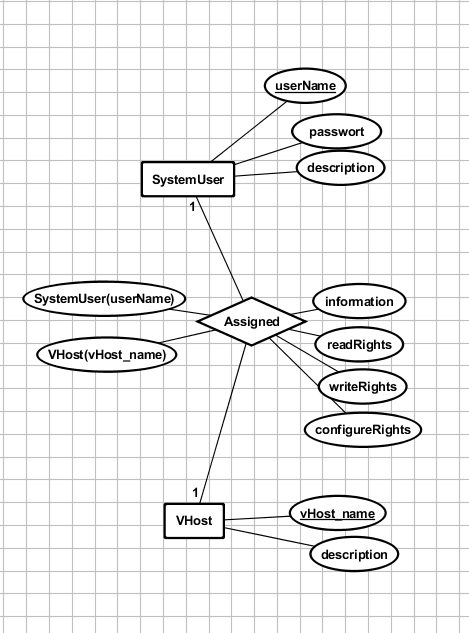
\includegraphics[width=0.5\textwidth]{Bilder/DBSchemaSystemUser.png}
	\caption{Datenbank ER Modellierung - Rabbit MQ System Data}
	\label{img:DBSchemaSystemUser}
\end{figure} 
Die Tabelle SystemUser  beinhaltet die LogIn Credentials und die Tabelle VHost lässt die Sicherung der RabbitMQ Informationen zu. 
Die n:m Beziehung zwischen System Usern und VHost wird in der Tabelle Assigned abgebildet. Hier lassen sich auch die jeweiligen Berechtigungen read, write und configure des Users auf der RabbitMQ Instanz hinterlegen.

\textbf{Wetter Daten ER Modell}
Damit die eingehenden Daten der WetterAPI  korrekt abgelegt werden können, sind Stammdaten in der Datenbank gepflegt. Neben den zur Verfügung stehenden Städten in der Tabelle City, werden auch die Standardwetterdaten (Tabelle DeaultWeather) aus der verwendeten WetterAPI hinterlegt. Jedes eingehende  Wetterdatenobjekt ist einer Stadt zugeordnet und referenziert ein DefaultWeather Eintrag.
Die User unserer Systemlösung können ebenfalls in der Datenbank gespeichert werden. Die Tabelle Subscribe beinhaltet die n:m Referenzen von Usern, welche bestimmte Städte beziehungsweise deren Wetterdaten abonniert haben. Jeder Eintrag in der Tabelle Subscribe besitzt zudem das Datum der Aktivierung des Abonnements. Abbildung … visualisiert das ER Modell der Wetterdatenspeicherung:
\begin{figure}[htbp]
	\centering
	\includegraphics[width=0.5\textwidth]{Bilder/DBSchemaWetterDaten.png}
	\caption{Datenbank ER Modellierung - Wetter Daten Modellierung}
	\label{img:DBSchemaWetterDaten}
\end{figure} 
Die Central Processing Unit, kurz CEP, errechnet anhand der eingehenden Wetterdaten verschiedene Benachrichtigungen (Alerts), welche über die MoM als Topic an die User verteilt werden. In der Datenbank können diese Alerts in Abhängigkeit der betroffenen Stadt gespeichert werden.

\subsection{Datenbank – JDBC Schnittstelle}
Der Zugriff und die Verwaltung der Datensätze nach dem, im vorherigen Kapitel beschrieben, Datenschema, ist in der Java Klasse  CadWeatherSystemDatabaseAPI realisiert. Diese Klasse lässt sich in alle Teilmodule unseres Gesamtsystems implementieren und bietet eine Schnittstellefunktionalität zur Verwendung der Datenbankinstanzen. In den Java Methoden, werden die MYSQL Kommunikationssatetments codiert als String über ein connection Objekt auf der Datenbank ausgeführt. Grundsätzlich stehen INSERT Operationen für alle Tabellen, sowie diverse SELECT Abfragemöglichkeiten zur Verfügung. Ziel dieser Struktur ist eine simple, vereinheitlichte Methodik zur Benutzung der Datenbankinstanzen.
Der Konstruktor der Klasse gibt dem Entwickler die Möglichkeit ein MYSQL Datenbankobjekt in die Schnittstelle einzubinden.

In der nachfolgenden Tabelle sind alle derzeit programierten Methoden aufgelistet.
Die INSERT  Methoden liefern das Feedback der Datenbankoperation in einem String zurück. Die Rückgabe ResultSet der select-Methoden beinhaltet die gefunden Datentupel der Abfrage.

{\bf GENERAL DB}
\begin{itemize}
\item checkDatabaseConnection()
\item java.sql.Connection getConnection()
\item setConnection(java.sql.Connection  databaseConnection)
\end{itemize}

{\bf CEP DB - INSERT}
\begin{itemize}
\item String insertDefaultWeather(int WeatherID, String main, String description, String icon_referenz)
\item String insertCity(int ZipCode, String cityName, Double logitude, Double latitude, int cityID)
\item String insertUser(String E_Mail, String userName, String passwort, int mainLocation)
\item String insertSubcribe(String E_Mail, int ZipCode)
\item String insertAlert(int ZipCode, Timestamp timestamp, String title, String code, String message)
\item String insertWeather(Timestamp TimeStamp, int ZipCode, int WeatherID, 
				double main_temp, double main_pressure, double main_humidity, double main_tempMin,
				double main_tempMax, double main_seaLevel, double main_grndLevel,
				String wind_direction, double wind_speed, double wind_deg, String clouds_desc, double rain_3h, 
				double snow_3h, 
				Timestamp sys_sunset, Timestamp sys_sunrise
				);)
\end{itemize}

{\bf CEP DB - SELECT }
\begin{itemize}
\item ResultSet selectUserByMail(String user_E_Mail)
\item ResultSet selectCityByZipCode(int city_ZipCode)
\item ResultSet selectDefaultWeatherByID(int defaultWeather_ID)
\item ResultSet selectAllWeatherByCityZipCode(int city_ZipCode)
\item ResultSet selectWeatherByCityAndDay(int city_ZipCode, Timestamp weatherDay)
\item ResultSet selectWeatherByCityAndTimePeriod(int city_ZipCode, Timestamp fromDate, Timestamp toDate) 
\item ResultSet selectSubscribeByUser(String user_E_Mail)
\item ResultSet selectSubscribeByCity(int ZipCode)
\item ResultSet selectUserPwByEMail(String E_Mail)
\end{itemize}

{\bf Rabbit MQ DB - Insert }
\begin{itemize}
\item String insertSystemUser(String userName, String password, String additionalDescription)
\item String insertVHost(String vHostName, String additionalDescription)
\item String insertAssigned(String systemUser_userName,String vHost_name, String additionalInformation, boolean readRights, boolean writeRights, boolean configureRights);
\end{itemize}

{\bf Rabbit MQ DB - SELECT }
\begin{itemize}
\item ResultSet selectVHostAll()
\item ResultSet selectSystemUserAll()
\item ResultSet selectSystemUserByUserName(String userName)
\item ResultSet ResultSet selectAssignedAll()
\end{itemize}



\subsection{Auswertungen & Nutzen der Databankspeicherung}
Die Datensätze können vielseitig genutzt werden. Zum einen hält die CEP Komponente unseres Systems die empfangen Wetterdaten der MoM bzw. der WetterAPI nur temporär. Gleiches gilt für erzeugte Benachrichtigungen in Form von Alerts.
Durch eine Sicherung in der Datenbank stehen die Wetterdaten unabhängig vom Status der CEP persistent zur Verfügung. 
Des Weiteren können verschiedene Auswertungen der Datensätze weitere Erkenntnisse bringen. 

\textbf{Wetter API User}
Durch die Protokollierung der Alerts lassen sich Statistiken über die Ereignisse und deren Verteilung aufstellen. Daraus könnten wir für die User beispielsweise Vorabwarnungen zukommen lassen. Außerdem könnte man den Usern auf lange Sicht gesehen Wettervergleiche bzw. Wetterentwicklungen bereitstellen.

\textbf{Cloud System Analyse}
Mithilfe des gespeicherten Datums der Aktivierung  von User Abonnements zu den jeweiligen Städten, lässt sich auch eine Prognose für unser System erstellen. Je nach Modell der Verteilung der gehosteten Komponenten unseres Systems  können wir aus den Datensätzen abschätzen, wie sich die Last auf unserem System entwickelt. 
Diese Prognosen können für eine Kostenabschätzung des Cloudsytsem wertvoll sein, um Ressourcen effizient einzusetzen und damit verbundene Kostenpunkte besser vorherzusagen.
Selbstverständlich ist der größte Vorteil einer Cloudlösung das dynamische Reagieren auf verschiedene Lastverhalten. Dennoch ist es im Rahmen von Businessmodellen notwendig zu wissen, welche Kosten an welcher Stelle entstehen beziehungsweise geplant werden können.

\subsection{AWS RDS Datenbankverfügbarkeit}
In Bezug auf die Performance spielt bei der Datenbank nur die Anzahl der CEP Calls eine Rolle. Dies führt je nach Szenario und Wetterveränderungen unterschiedlich viele I/O Operationen aus. Dennoch würde unser WetterAPI System selbst bei extrem hohen Userzahlen keine Datenlast liefern, welche die Datenbank an ihre Grenze bringen könnte. Das Bottleneck unseres Systems sind die Instanzen der CEP. Im Rahmen unseres Projektes ist die Skalierung des Datenbank Services nicht eingerichtet, da zusätzliche oder skalierte Datenbankinstanzen mit hohen Kosten verbunden sind, da die benötigten Konfigurationen nicht im Umfang des AWS Trialkontingents enthalten sind. Ganz wichtig ist die Tatsache, dass das Starten einer weiteren Instanz das kostenlose Kontigent an Ressourcen aufhebt. Aus eigener Erfahrung wissen wir, wie sich ein solches Szenario zu einer gewissen Kostenfalle entwickeln kann.
An dieser Stelle sollen dennoch die Möglichkeiten der Datenbankverfügbarkeit in Bezug auf den AWS RDS Dienst beschrieben werden.

\textbf{Vertikale Skalierung}
Die Datenbank empfängt viele write-Operationen, weshalb eine vertikale Skalierung in unserem Fall der beste Ansatz wäre. Amazon bietet in seinem Service RDS (Relationale Datenbank Services) automatische Skalierungsoptionen an. So lassen sich verschiedene Monitoring Parameter (z.B. CPU Auslastung) einstellen, welche beim Erreichen eines Grenzwertes automatisch weitere Kapazitäten zur Verfügung stellt. Der Datenbankinstanz können je nach genutzer Datenbankengine bis zu 32 vCPU's mit 244GB RAM uns bis zu 64TB Datenspeicher zugeschaltet werden. Ein minimaler Nachteil ist eine kurze Downtime Phase in der die neuen Ressourcen eingebunden werden. Es gehen aber keine gespeicherten Daten verloren, sodass man in die Write Operationen der CEP im internen Speicher der CEP halten und bei erneuter Datenbankverfügbarkeit an den RDS Dienst übergeben könnte.

\textbf{Horizontale Skalierung}
Eine horizontale Skalierung eignet sich vor allem bei Applikationen mit einem hohen Anteil an read-Operationen. Hierfür kann man beispielsweise den Amazon Container Service verwenden. Auch hier kann man Amazon konfigurieren, bei einem gewissen Lastverhalten, über einen Dockercontainer eine weitere Instanz aufzuziehen.
Eine weitere Möglichkeit für eine horizontale Skalierung, sind Replica Objekte. Ein Replica Objekt bildet den Aufbau und den Inhalt einer Datenbankinstanz ab und steht für weitere Instanzdeployments zur Verfügung. 

\textbf{Ausfallsicherheit}
Für die Ausfallsicherheit bietet der AWS RDS Dienst die Option Multi-AvailabilityZone. Wenn die Option aktiviert wird, erstellt Amazon eine synchronisierte Datenbankinstanz in einer anderen Region bzw. in einem anderen Rechenzentrum. Beim Ausfall der aktiven Datenbankinstanz wird innerhalb einer Minute die synchrone Datenbankinstanz zugeschaltet und das DNS angepasst, damit sich aus Applikationssicht nichts verändert.


\subsection{12 Faktor App}\label{12FactorApp}
In diesem Absatz wird dargestellt, ob und wie die Anforderungen umgesetzt wurden.


\begin{table}[!ht]
  \centering
    \begin{minipage}{17cm}
      \centering
      \begin{tabular}{*{3}{|l|p{3.0cm}|p{7.0cm}}}\hline
      \multicolumn{4}{|c|}{\cellcolor[RGB]{200,200,200}Validierung nach "12 Faktor APP"} \\\hline
     \textbf{ID}&\textbf{Anforderung}&\textbf{Validierungs Element}&\textbf{Erfüllt}\\\hline
     1.&Codebase&Andere Komponenten sind nur für das Testszenario da. Deployment verschiederner Versionen über Repo möglich&Ja\\
      \hline
     2.&Abhängigkeiten&Keine Abhängigkeiten zu anderen Komponenten&Nein\\
     \hline
     3.&Konfiguration&Konfigurationsdatei wird beim Start des Containers aufgerufen und schränkt den Gast-Zugang auf localhost ein. Credentials werden über Umgebungsvariablen im Amazon Container Service (ACS) gepflegt.&Ja\\
     \hline
     4.&Unterstützende Dienste&Keine unterstützenden Dienste vorhanden&Nein\\
     \hline 
     5.&Build, release, run& Könnte durch Jenkins verwaltet werden. Da die MOM keine regelmäßigen Update-Zyklen durchläuft, wurde darauf verzichtet.&Möglich,\- nicht aktiv\\
     \hline
     6.&Prozesse&Der Start des RabbitMQ wird durch das init-Skript im Dockerfile gesteuert. Dieses wird durch dem CMD-Befehl automatisch ausgerufen, so dass der Anwender nur den Task im ACS starten muss (ref{acs}).&Ja\\
     \hline
      7.&Bindung an Ports&Notwendige Ports werden über die EXPOSE-Befehle im Dockerfile deklariert. Das Mapping dieser Ports wird in den Container-Einstellungen von ACS definiert. &Ja\\
     \hline
      8.&Nebenläufigkeit&Die Skalierung kann über ACS erfolgen. ACS ist bereits hoch skalierbar und bietet dem Verwalter des Containers die Konfiguration der Skalierung an. So können Minimum- und Maximum-Tasks sowie eine gewünschte Anzahl an Tasks definiert werden. Die Anzahl der laufenden Tasks bestimmt die Anzahl der laufenden Instanzen. Im verwendeten Nutzungsplan von ACS ist eine Instanz im Mittel über einen Monat verteilt kostenlos verfügbar.&Ja\\
     \hline
      9.&Einweggebrauch&Der Container kann schnell stoppt und gestartet werden. Durch Probleme mit der Rabbitmq-eigenen Datenbank besteht dann allerdings die Gefahr, im laufenden Betrieb hinzugefügte Nutzer neu hinzufügen zu müssen, da diese bei Rabbitmq auf den Namen des Hosts gespeichert werden und sich dieser beim Neustart des Containers ändert. Ein Workaround wurde entwickelt, dieser aktualiert aber lediglich das Init-Skript und fügt diesem die Nutzer automatisch hinzu. Dadurch muss beim Neustart auch das Skript aktualisiert werden. &Teilweise\\
     \hline
     10.&Dev-Prod-Vergleichbarkeit&Containerisierung durch Docker (\ref{Docker}).&Ja\\
     \hline     
     11.&Logs&Das Docker-Image von Rabbitmq gibt die Log standardmäßig über Stdout (tty) aus&Ja\\
     \hline
     12.&Admin-Prozesse&Automatische Ausführung eines Skripts beim Containerstart&ja\\
     \hline
      \end{tabular}
   \caption{Validierung der CEP nach "12 Faktor APP"}\label{tab:AnforderungenCEP}
    \end{minipage}
\end{table}


\end{document}